%%%%%%%%%%%%%%%%%%%%%%%%%%%%%%%%%%%%%%%%%%%%%%%%%%%%%%%%%%%%%%%%%%%%%%%%%%
% File: Lecture_1.tex
% Authors: James Kress
% Date: February 1, 2014
% Description: 
%%%%%%%%%%%%%%%%%%%%%%%%%%%%%%%%%%%%%%%%%%%%%%%%%%%%%%%%%%%%%%%%%%%%%%%%%%

%<<<<<<<<<<<<<<<<<<<<<<<<<<<<<<<<<<<<<<<<<<<<<<<<<<<<<<<<<<<<<<<<<<<<<<<<<<<<<%
% Document package information
%>>>>>>>>>>>>>>>>>>>>>>>>>>>>>>>>>>>>>>>>>>>>>>>>>>>>>>>>>>>>>>>>>>>>>>>>>>>>>%
\documentclass[xcolor=dvipsnames]{beamer} 
%%%%%%%%%%%%%%%%%%%%%%%%%%%%%%%%%%%%%%%%%%%%%%%%%%%%%%%%%%%%%%%%%%%%%%%%%%
% File: _TeXdefs.tex
% Author: James Kress
% Date: January 25, 2014
% Description: A tex file containing the \usepackage declarations, and
%			   other document critial style settings.
%%%%%%%%%%%%%%%%%%%%%%%%%%%%%%%%%%%%%%%%%%%%%%%%%%%%%%%%%%%%%%%%%%%%%%%%%%

%-----------Package imports
\usepackage{graphicx}
\usepackage{pgfpages}
\usepackage{tikz}
\usepackage{latexsym}
\usepackage{verbatim}
%//////////END package imports


%----------Style elements
\useoutertheme{infolines} 
\usetheme{Frankfurt} 
\usepackage{../theme/beamercolorthemeoregon}
\setbeamertemplate{sections/subsections in toc}[default]
\setbeamertemplate{footline}
{
\leavevmode%
  \hbox{%
  \begin{beamercolorbox}[wd=.3\paperwidth,ht=2.25ex,dp=.75ex,center]{institute in head/foot}%
    \usebeamerfont{institute in head/foot}\insertshortinstitute
  \end{beamercolorbox}%
    \begin{beamercolorbox}[wd=.4\paperwidth,ht=2.25ex,dp=.75ex,center]{title in head/foot}%
      \usebeamerfont{title in head/foot}\insertshorttitle
    \end{beamercolorbox}%
  \begin{beamercolorbox}[wd=.3\paperwidth,ht=2.25ex,dp=.75ex,center]{date in head/foot}%
    \usebeamerfont{date in head/foot}\insertshortdate\hspace*{3em}
    \insertframenumber{} / \inserttotalframenumber\hspace*{1ex}
  \end{beamercolorbox}}%
  \vskip0pt%
}
%/////////END style elements


%---------Command Declarations
\DeclareGraphicsExtensions{.pdf, .jpeg, .png, .jpg}
\graphicspath{ {../images/} }
\newcommand{\className}{\text{CIS 410/510} \\ \text{Parallel Computing}}
\newcommand{\departmentName}{\textit{Department of Computer and 
									Information Science \\ University of Oregon}}
%/////////END command declarations


%---------Setup pdf properties
\hypersetup{
	pdfusetitle=true,
    bookmarks=true,         	% show bookmarks bar?
    unicode=false,          	% non-Latin characters in Acrobat’s bookmarks
    pdftoolbar=true,        	% show Acrobat’s toolbar?
    pdfmenubar=true,        	% show Acrobat’s menu?
    pdffitwindow=false,     	% window fit to page when opened
    pdfstartview={Fit},   		% fits the width of the page to the window    
    pdfauthor={},     % author
    pdfsubject={Parallel Programming},   	% subject of the document
    pdfcreator={},   			% creator of the document
    pdfproducer={}, 			% producer of the document
    pdfkeywords={University of Oregon, parallel programming}, 
    pdfnewwindow=true,      	% links in new window
    colorlinks=true,       		% false: boxed links; true: colored links
    linkcolor=white,          	% color of internal links
    hidelinks,
    citecolor=green,        	% color of links to bibliography
    filecolor=magenta,      	% color of file links
    urlcolor=cyan,           	% color of external links
    linktoc=page,
    pageanchor = true
}
%//////////END setup pdf properties


%END ALL


%<<<<<<<<<<<<<<<<<<<<<<<<<<<<<<<<<<<<<<<<<<<<<<<<<<<<<<<<<<<<<<<<<<<<<<<<<<<<<%
% END Document package information
%>>>>>>>>>>>>>>>>>>>>>>>>>>>>>>>>>>>>>>>>>>>>>>>>>>>>>>>>>>>>>>>>>>>>>>>>>>>>>%

%=============================================================================%
% Begining: Title Page Material
%=============================================================================%
\begin{document}
	\title[Collective Pattern]{Collective Pattern}
	\author[]{\className}
	\institute[\className]{\departmentName}
	\date{} 

	\titlegraphic{\centering 
		$\vcenter{\hbox{
\includegraphics[height=.31in,width=2.0in]{oregonLogo}}}$
	}

	\begin{frame}
		\maketitle
	\end{frame}
	
	\begin{frame}{Developer Training}
		\begin{center}
			
\includegraphics[width=0.4\textwidth]{images/OSNAP_logo} 
			
			Collective Pattern
			
			Executive Password Recovery
		\end{center}
	\end{frame}
	
	\begin{frame}{Executive Password Recovery}
		\begin{columns}
			\begin{column}{0.5\textwidth}
				  Our previous weeks' endeavors have emboldened management in their efforts to avoid
          work
					\\~\\
          Executives have passwords they must change weekly, these are too valuable to simply
          be hashed. They must be encrypted by a series of keys stored in a set of 
          undisclosed locations. For this, they will need an encryption tool capable
          of taking the set of encryption keys and encrypting a password. Having all keys
          also enables a password to be recovered, preventing management from needing to
          remember theirs.
			\end{column}
			\begin{column}{0.5\textwidth}
				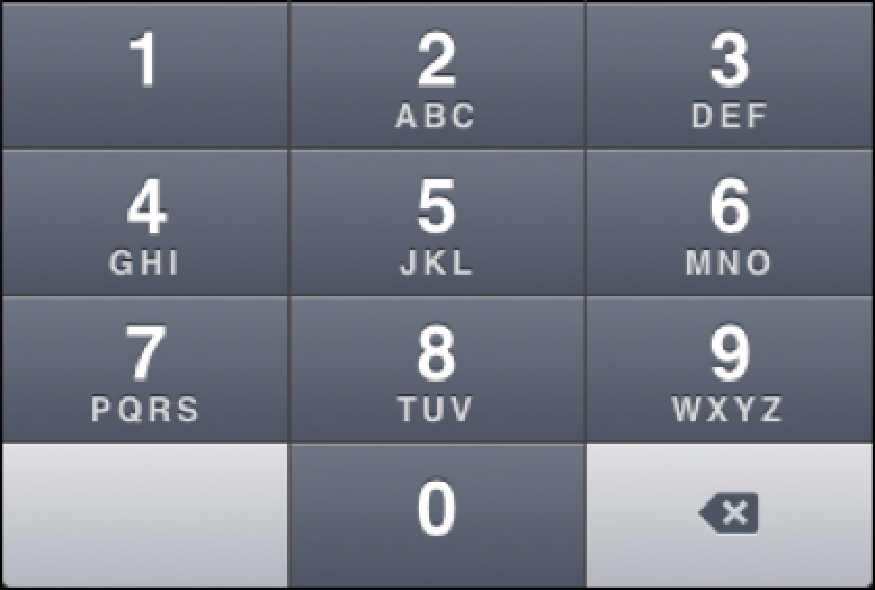
\includegraphics[width=\textwidth]{images/keypad}
			\end{column}
		\end{columns}
	\end{frame}
	
  \begin{frame}{Encryption Algorithm - Multi Key Xor}
		\begin{columns}
			\begin{column}{0.5\textwidth}
          XOR based encryption is a class of encryption algorithms in which the encryption
          and decryption keys are the same
					\\~\\
			    Each bit of the string is compared to the corresponding bit in a string of key
          bits for any number of keys. These keys can and will have different lengths,
          some combinations of key lengths lend themselves to trivial solutions. We will
          not make things that easy on the aliens. For messages longer than the length of
          our keys we will cycle back to the beginning of a key when we run out of key bits
      \end{column}
			\begin{column}{0.5\textwidth}
				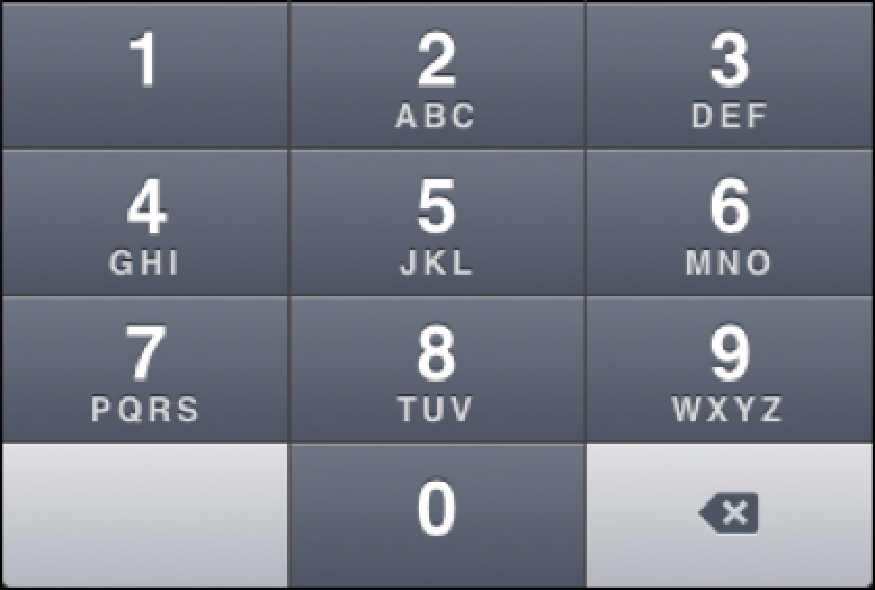
\includegraphics[width=\textwidth]{images/keypad}
			\end{column}
		\end{columns}
	\end{frame}
	
	\begin{frame}{Basic Solution}
		\begin{itemize}
			\item You will be provided a password
			\item Give the software a number of keys to generate
			\item Software generates the given number of keys
			\item Software prints plaintext, then prints encoded text, then prints decrypted text to prove results
			\item \href{http://ix.cs.uoregon.edu/~dellswor/410}{\url{http://ix.cs.uoregon.edu/~dellswor/410}}
		\end{itemize}
	\end{frame}
	%--- Next Frame ---%
	
  \begin{frame}{Collective Reduce Operation}
		\begin{columns}
			\begin{column}{0.5\textwidth}
				\begin{itemize}
					\item N atomic data units, one output (a Gather Operation)
					\item Binary operation applied across inputs to produce the result
					\item Example: adding all input integers in a list to create output sum
          \item We will be xor'ing an input bit with a set of key bits to create output bit
				\end{itemize}
			\end{column}
			\begin{column}{0.5\textwidth}
				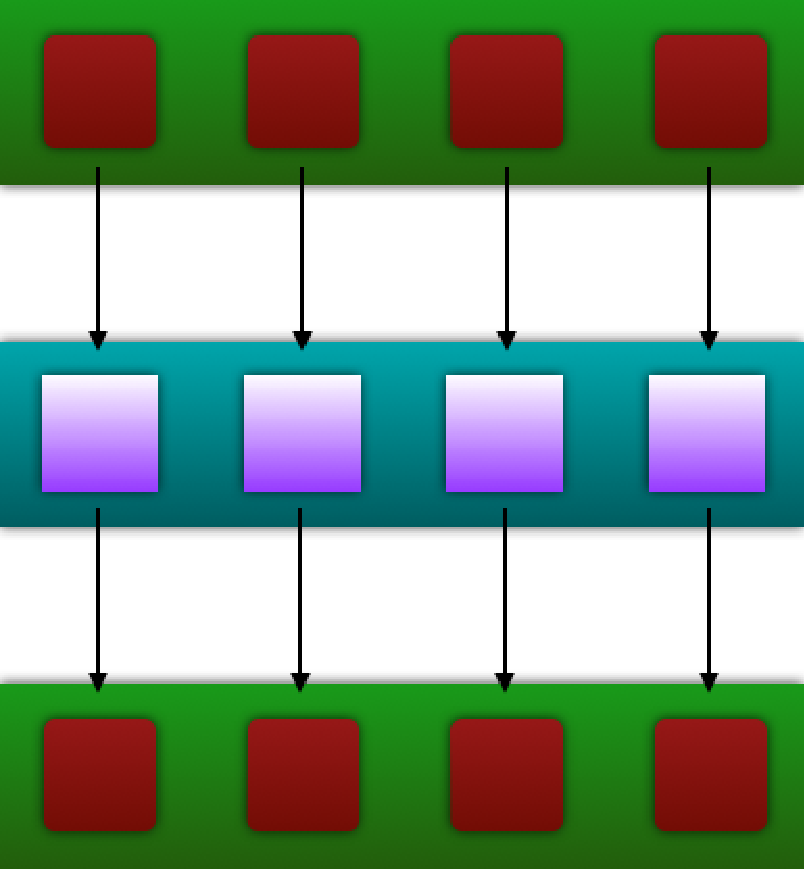
\includegraphics[width=\textwidth]{images/mapPattern}
			\end{column}
		\end{columns}
	\end{frame}
	
	
	\begin{frame}{Parallel Multiple Key Xor}
		\begin{itemize}
			\item Our solution is way too slow
			\item If only we had a team of developers to parallelize it...
		\end{itemize}
	\end{frame}
	
	\begin{frame}{Multiple Passwords - Example code}
		\begin{itemize}
      \item Example code is stored on Mist
      \item Get into a directory you store source in 
			\item On Mist: run "cp -r /home/users/poliadz/OpenmpPasswordCracker ."
		\end{itemize}
	\end{frame}
  
  \begin{frame}{Key Points - Map}
		\begin{itemize}
      \item Concept: apply the same operation to multiple data elements, producing a single output
      \item Design: Challenge in map is ensuring operations do the same amount of work
			\item Identifying the correct parallelization is key to performance
		\end{itemize}
	\end{frame}
	
	%--- Next Frame ---%

\end{document}
%END ALL

